
\section{Introduction}
\label{sec:introduction}

In this paper, we investigate \emph{tiebreaking strategies} for cost-optimal \astar.
% In optimal search, tiebreaking strategies does not affect the optimality
% of the search algorithms because they only affect the node expansion
% order among the nodes with the same $f$-cost.
% \subsection{Tiebreaking for \astar}
% This paper is organized as follows.
% After defining some notations in \refsec{sec:preliminaries}, 
% We first investigate the conventional
% tiebreaking strategies for the optimal search using \astar.
\astar is the standard search algorithm for finding an optimal-cost path from an initial state $s$ to some goal
state $g \in G$ in a search space represented as a graph \cite{hart1968formal}.
It expands the nodes in the best-first order of $f(n)$ until up to $f^*$,
where $f(n)$ is a lower bound of the cost of the shortest path that contains a node $n$ and $f^*$ is the optimal cost.
% 
In many combinatorial search problems, the size of the last layer $f(n)=f^*$ of the search , called \emph{final plateau},
accounts for a significant fraction of the effective search space of \astar.  \refig{fig:plateau-noh}
(\refpage{fig:plateau-noh}) compares the number of states in this final plateau with $f(n) = f^*$ (y-axis)
vs. $f(n) \leq f^*$ (x-axis) for 1104 problem instances from the International Planning Competition (IPC1998-2011).
For many instances, a large fraction of the nodes in the effective search space have $f(n)=f^*$: The points
are located very close to the diagonal line ($x=y$), indicating almost all states with $f(n) \leq f^*$ have cost
$f^*$.

\refig{fig:plateau-0} depicts the conceptual view of these phenomenon.
% 
A naive view of the search space (left) would consider the space searched by \astar as
a thin layer of final plateau $f(n)=f^*$ surrounding a large number of closed nodes with $f<f^*$.  This view is
intuitive, and may accurately describe some real, practical search spaces such as 2D path finding on an explicit
graph. It also gives a foundation to some family of search algorithms like Frontier Search
\cite{korf1999divide,korf2000divide}, which tries to reduce the memory requirement by discarding the information on
$f<f^*$, which may work if $f<f^*$ is large.
% 
However, for many combinatorial search problems,
the figure on the right is a more accurate depiction -- the  search space has a large plateau for $f=f^*$.
In fact, Iterative Deepening approaches \cite{korf1985depth} assume this type of search space
where this final frontier is quite huge and the cost of re-evaluating $f<f^*$ is limited.
Classical planning problems in IPC benchmarks are clearly the instances of such combinatorial search problems.
\todo*{The fact that the last layer of search dominates the search was the motivation for Frontier Search and its numerous variants, so the SoCS community has been well aware of this --- SoCS community considers the opposite. Frontier search would not gain advantage in the planning domains because the number of nodes being forgotten is low compared to the size of the plateau.}

\begin{figure}[htbp]
  \centering
  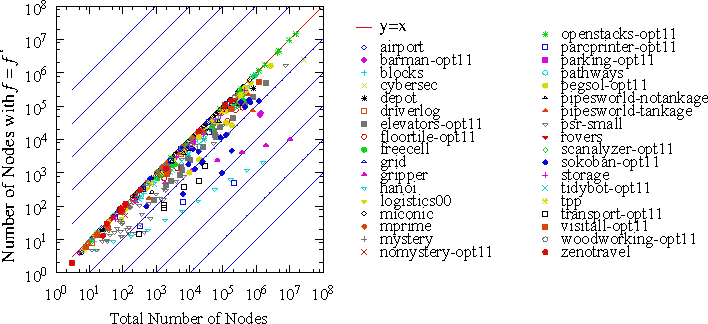
\includegraphics{tables/aaai16-frontier/aaai16prelim3/lmcut_frontier_noh-front.pdf}
 \caption{
 The number of nodes with $f=f^*$ (y-axis) compared to the
 total number of nodes in the search space (x-axis) with $f\leq f^*$ on 1104 IPC benchmark problems.
 This experiment uses a modified Fast Downward with \lmcut which 
 continues the search within the current $f$ after any optimal solution is found.
 This effectively generates all nodes with cost $f^*$.
  }
 \label{fig:plateau-noh}
\end{figure}

\begin{figure}[htbp]
  \centering
  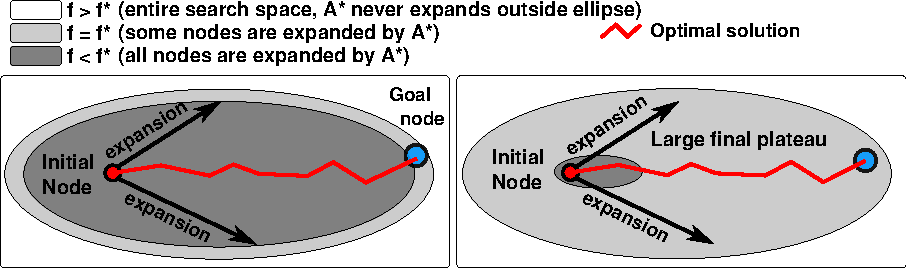
\includegraphics{img/astar/plateau-0.pdf}
 \caption{(Left) Naive understanding of the search space of \astar, which only holds for some limited domains. (Right) The reality of search spaces of combinatorial problems. Plateau containing the optimal goals ($f=f^*$) is large, and it even accounts for most of the search effort required by \astar.
  }
 \label{fig:plateau-0}
\end{figure}

In the majority of such IPC problem domains where the 
the last layer ($f(n)=f^*$) accounts for a significant fraction of the effective search space, a
\emph{tiebreaking strategy}, which determines which node to expand among nodes with the same $f$-cost,
can have a significant impact on the performance of \astar.
It is widely believed that among nodes with the same $f$-cost,
ties should be broken according to $h(n)$, i.e.,
nodes with smaller $h$-values should be expanded first.  While this is a
useful rule of thumb in many domains, it turns out that tiebreaking
requires more careful consideration, particularly for problems where
most or all of the nodes in the last layer have the same $h$-value.

We empirically evaluate the existing, commonly used, standard
tiebreaking strategies for \astar (\refsec{sec:eval-common-strategies}).
We show that:

\begin{enumerate}
 \item A Last-In-First-Out (\lifo) criterion tends to be more efficient
       than a First-In-First-Out (\fifo) criterion.
 \item Tiebreaking according to the heuristic value $h$, which
       frequently appears in the heuristic search literature, has little
       impact on the performance as long as \lifo default criterion is used 
       --  in other words, a \lifo tiebreaking policy is sufficient for most IPC domains.
 \item There are significant performance differences among tiebreaking strategies
       when domains include zero-cost actions. This is true even when $h$-based tiebreaking is used.
\end{enumerate}

While there are relatively few domains with zero-cost actions in the IPC
benchmark set, we argue that zero-cost actions naturally occur in
practical cost-minimization problems. Therefore we introduce a new set of
benchmarks called \emph{zerocost domains}
(\refsec{sec:zerocost-domains}).  We empirically show that these
zerocost domains have the different search space structure and different
problem difficulty from those of the original domains.

In order to solve such problems more efficiently, we propose and
evaluate \emph{depth diversification}, a new
tiebreaking method based on the notion of a node's \emph{depth} within a plateau,
which corresponds to the number of steps from the ``entrance'' to
the plateau (\refsec{sec:depth},
\refsec{sec:depth-based-evaluation}). We also evaluate an
admissible tiebreaking strategy which uses the distance-to-go estimate, a heuristic function which treats every actions
to have the unit costs (\refsec{sec:distance-to-go}).
Although distance-to-go estimates are inadmissible,
it does not harm the admissibility of entire search as long as it is used only for tiebreaking.
% 
In these sections, we empirically show that:
\begin{enumerate}
 \item Our new depth-based diversification strategy significantly improves upon the 
       standard tiebreaking strategies.
 \item Tiebreaking using distance-to-go variations of \lmcut, \mands and \ff heuristics
       significantly improves the standard tiebreaking strategies.
       \todo*{listing 3 points regarding d2go might give the wrong impression that this paper is about d2go. combine some of the d2go bullets, or add another depth-related bullet?}
 % \item Distance-to-go variations of \emph{inadmissible} heuristics
 %       (\ff) further improves the performance by an order of magnitude.
 \item Combining depth-based diversification with distance-to-go heuristics 
       further improves the performance.
\end{enumerate}

Finally, in \refsec{sec:discussion}, we discuss the implications of these results.
We offer a new perspective to admissible \astar search:
Admissible \astar can be seen as a series of satisficing searches on each plateau,
and thus the problem of tiebreaking can be reduced to satisficing search techniques.
% 
In order to strengthen the connection between tiebreaking and satisficing search,
we also show a preliminary result of the depth diversification,
which was shown to improve tiebreaking performance,
also improves satisficing search using Greedy Best First Search (GBFS).
We further discuss the future direction, related works, and close the article.

\textbf{
Note for reviewers:
This paper is a significantly extended version of the AAAI-16 paper by
the same authors. The addition to the conference paper is the following:
\begin{enumerate}
 \item Introduction of deterministic depth-based diversification
       strategy (as opposed to the randomized version in the conference
       paper), and its theoretical analysis in \refsec{sec:depth}. We
       also added thorough empirical analysis in
       \refsec{sec:depth-based-evaluation} that are not included in the
       conference version.
 \item Empirical analysis of distance-to-go estimates in
       \refsec{sec:distance-to-go}.  Also, we included an empirical
       evaluation of the use of inadmissible FF heuristics as part of
       tiebreaking criterion, and its combination with the
       depths metric thereof.
 \item New perspective to \astar and the preliminary results on the use
       of depth for satisficing planning (\refsec{sec:discussion}).
\end{enumerate}
}

